\documentclass[lang=cn,10pt,green]{elegantbook}
\usepackage{float}
\usepackage{subfigure}
\usepackage[normalem]{ulem} % \sout{想加删除线的中文}
\usepackage{wrapfig}
\usepackage{extarrows}
\newcommand{\incfig}[1]{%
\def\svgwidth{\columnwidth}
\import{./figures/}{#1.pdf_tex}
}



\renewcommand{\proofname}{\indent Pr}

\newcommand{\argmin}[1]{\underset{#1}{\arg \min}\ }
\newcommand{\ceil}[1]{\left\lceil #1 \right \rceil }
\newcommand{\norm}[1]{\left \Vert #1 \right \Vert}
\newcommand{\tform}[1]{\left \Vert #1 \right \Vert_2}
\newcommand{\tnorm}[1]{\left \Vert #1 \right \Vert_2}
\newcommand{\onorm}[1]{\left \Vert #1 \right \Vert_1}
\newcommand{\abs}[1]{\left|#1 \right|}
\newcommand{\var}[1]{\text{Var}\left[ #1\right]}
\newcommand{\xk}[1]{\left( #1\right)} 
\newcommand{\zk}[1]{\left[ #1\right]} 
\newcommand{\dk}[1]{\left\{ #1\right\}} 
\newcommand{\bd}[1]{\bold{#1}}

%量子力学符号------
\newcommand{\xde}{\text{Schrödinger}}
\newcommand{\avg}[1]{\left \langle #1 \right \rangle}
\newcommand{\lvec}[1]{\left \langle #1 \right |}
\newcommand{\rvec}[1]{\left | #1 \right \rangle}


\newtheorem{lproof}{证明}[section]
\newtheorem{tuilun}{推论}
\newtheorem{eg}{例}[section]
\newtheorem{solve}{解}[section]
\newcommand\ii{\textup{i}}
\newcommand\dd{\mathrm{d}}


%自定义数学符号
\newcommand{\diag}{\textup{diag}}
\newcommand{\Frobenius}[1]{\left\Vert #1 \right\Vert}
\newcommand{\fform}[1]{\left\Vert #1 \right\Vert_F}
\newcommand{\parr}[2]{\frac{\partial #1}{\partial #2}}%一阶偏微分
\newcommand{\parrr}[2]{\frac{\partial^2 #1}{\partial #2^2}}%二阶偏微分
\newcommand{\lap}[1]{\parrr{#1}{x} + \parrr{#1}{y} = 0}%二元拉普拉斯方程
\newcommand{\ddd}[2]{\frac{\textup{d} #1}{\textup{d} #2}}%微商
\newcommand{\dddd}[2]{\frac{\textup{d}^2 #1}{\textup{d} #2^2}}%微商

%二重以上环路积分,强迫症了属于是
\def\ooint{{\bigcirc}\kern-11.5pt{\int}\kern-6.5pt{\int}}
\def\oooint{{\bigcirc}\kern-12.3pt{\int}\kern-7pt{\int}\kern-7pt{\int}}


\newcommand{\tu}{\textup}
\newcommand{\ol}[1]{$\overline{#1}$}
\newcommand{\re}[1]{\textup{Re}(#1)}
\newcommand{\im}[1]{\textup{Im}(#1)}
\newcommand{\fa}{\forall}
\newcommand{\ex}{\exists}
\newcommand{\st}{\textup{  s.t. }}
\newcommand{\ve}{\varepsilon}
\newcommand{\disp}{\displaystyle}
\newcommand{\chj}{\textup{Cauchy}积分公式}
\newcommand{\res}[1]{\textup{Res}\left(#1\right)}
\newcommand{\mysum}[1][n]{\sum_{i = 1}^{#1}}%求和
\newcommand{\series}[1]{\sum_{n = 0}^{\infty} #1_{n}}%级数
\newcommand{\seriesa}[1]{\sum_{n = 0}^{\infty} \left| #1_{n}\right|}%绝对级数
\newcommand{\fseries}[1]{\sum_{k = 1}^{\infty} #1_k (z)}

\newcommand*{\num}{pi}

%书写横线
\newcommand{\horrule}[1]{\rule[0.5ex]{\linewidth}{#1}} 	% Horizontal rule

\title{Introduction to Computer Vision Notes}
\subtitle{授课教师:\href{https://hughw19.github.io}{王鹤}}
\author{林晓疏, \href{https://lyt0112.com/}{梁宇桐}, \href{https://iculizhi.github.io/}{徐靖}}
\institute{PKU EECS}
\version{2025 Spring}
\bioinfo{声明}{\textcolor{red}{请勿用于个人学习外其他用途!}}
\extrainfo{个人笔记,如有谬误,欢迎指正!\\ 联系方式:2200012917@stu.pku.edu.cn}

\setcounter{tocdepth}{3}

% 自定义封面元素
\cover{cover.jpg}
\logo{logo-blue.png}

% 本文档命令
\usepackage{array}
\newcommand{\ccr}[1]{\makecell{{\color{#1}\rule{1cm}{1cm}}}}

% 修改标题页的橙色带
% \definecolor{customcolor}{RGB}{32,178,170}
% \colorlet{coverlinecolor}{customcolor}
\setcounter{tocdepth}{3} % 设置目录深度
\begin{document}

\maketitle
\frontmatter

% \tableofcontents

\mainmatter

\chapter{Line Fitting}

\begin{introduction}[Keywords]
    \item 最小二乘法 Least Square Method
    \item 奇异值分解 Singular Value Decomposition (SVD)
    \item 随机抽样一致算法 RANdom SAmple Consensus (RANSAC)
    \item 霍夫变换 Hough Transform
    \item 鲁棒性 Robustness
    \item 离群点 Outliers
    \item 内点 Inliers
\end{introduction}

\section{Least Square Method}

最小二乘法想必都熟知

\begin{figure}[htbp]
    \centering
    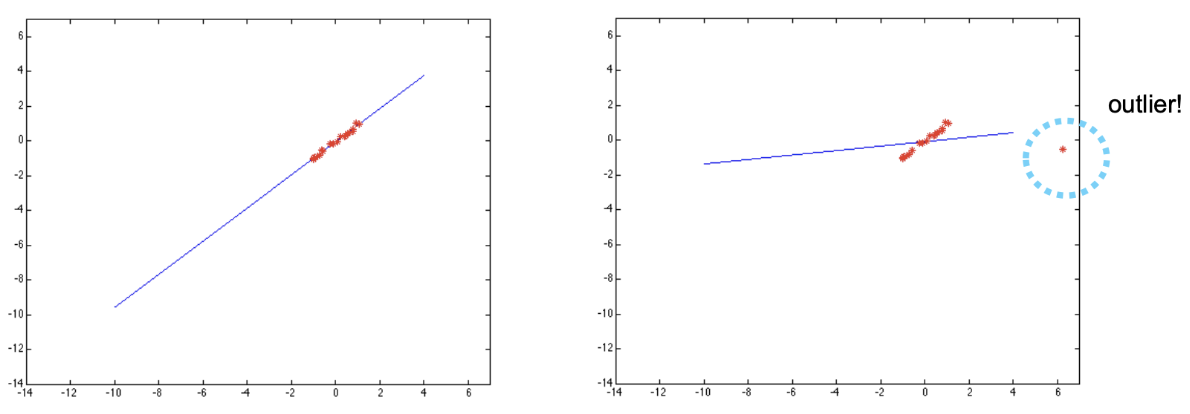
\includegraphics[width=0.8\textwidth]{figures/not_roboust_outliner.png}
    \caption{Least Square Method is not robust to outliers}
\end{figure}

对细微噪声\textbf{鲁棒(robust)}, 但是对于\textbf{离群点(Ouliers)}敏感.

\href{http://faculty.bicmr.pku.edu.cn/~wenzw/bigdata/matrix-cook-book.pdf}{Matrix Cookbook} : 记录了很多矩阵求导的公式

\section{Singular Value Decomposition (SVD)}

SVD 这里的作用在于, 对给定一组数据点, 找到最适配的 k 维子空间, 使得所有数据点到这个子空间的距离最小. 这里我认为王鹤老师讲解地不够本质, 但 SVD 本身非常基础, 可以自行查阅资料.

\newpage
\section{RANSAC}


RANSAC : RANdom SAmple Consensus

Idea: we need to find a line that has the largest supporters (or inliers)

\begin{definition}[RANSAC loop]
    假设这个直线 (平面) 需要两个 (n个) 点来确定 : 

    \begin{enumerate}
        \item 随机选择 k 组能确定这个直线的点,也就是在所有点里面选出一个 $k\times 2$ 的矩阵
        \item 对每一组点计算出一条直线 (SVD)
        \item 对每一组点的直线计算出所有点到这条直线的距离,如果小于阈值,则认为这个点是这条直线的 inlier
        \item 找到最大的 inlier 数量的直线,如果大于阈值,则认为这条直线是最优的
        \item 对这个最优的直线,用这个直线所有的 inlier 重新计算一次直线
        \item 重复上述步骤, 直到 inlier 数量不再增加
    \end{enumerate}
    
\end{definition}
\begin{note}
    实际上从今天来看这个 loop 不需要, 因为我们可以并行地提出所有假设 (Hypothesis), 这里王鹤老师留作作业.
\end{note}

\section{RANSAC calculation}
\begin{problem}
假设我们有所有 inliner 占比为 $w$ 的先验知识,同时希望有不低于 $p$ 的概率能够找到一个最优的直线,那么我们需要多少次迭代呢?
\end{problem}
\begin{proof}
注意到, 
\begin{equation}
\mathbf{\Pr}\text{[一组点全部是inliner]} = w^n
\end{equation}

如果一组点中有一个点是 outliner,那么我们称这组点 fail.

\begin{equation}
\mathbf{\Pr}\text{[k组点全部fail]} = {(1-w^n)}^k
\end{equation}

我们希望 k 组点全部 fail 的概率小于 $1-p$.

\begin{equation}
{(1-w^{n})}^k < 1-p
\Rightarrow
k > \frac{\log(1-p)}{\log(1-w^n)}
\end{equation}
\end{proof}

\newpage
\section{Hough Transform}

其实就是把一条直线从实际空间的表示转换到参数空间的表示. 但是如果存在垂直的直线, 可能需要考虑使用极坐标来作为参数空间.

\begin{figure}[htbp]
    \centering
    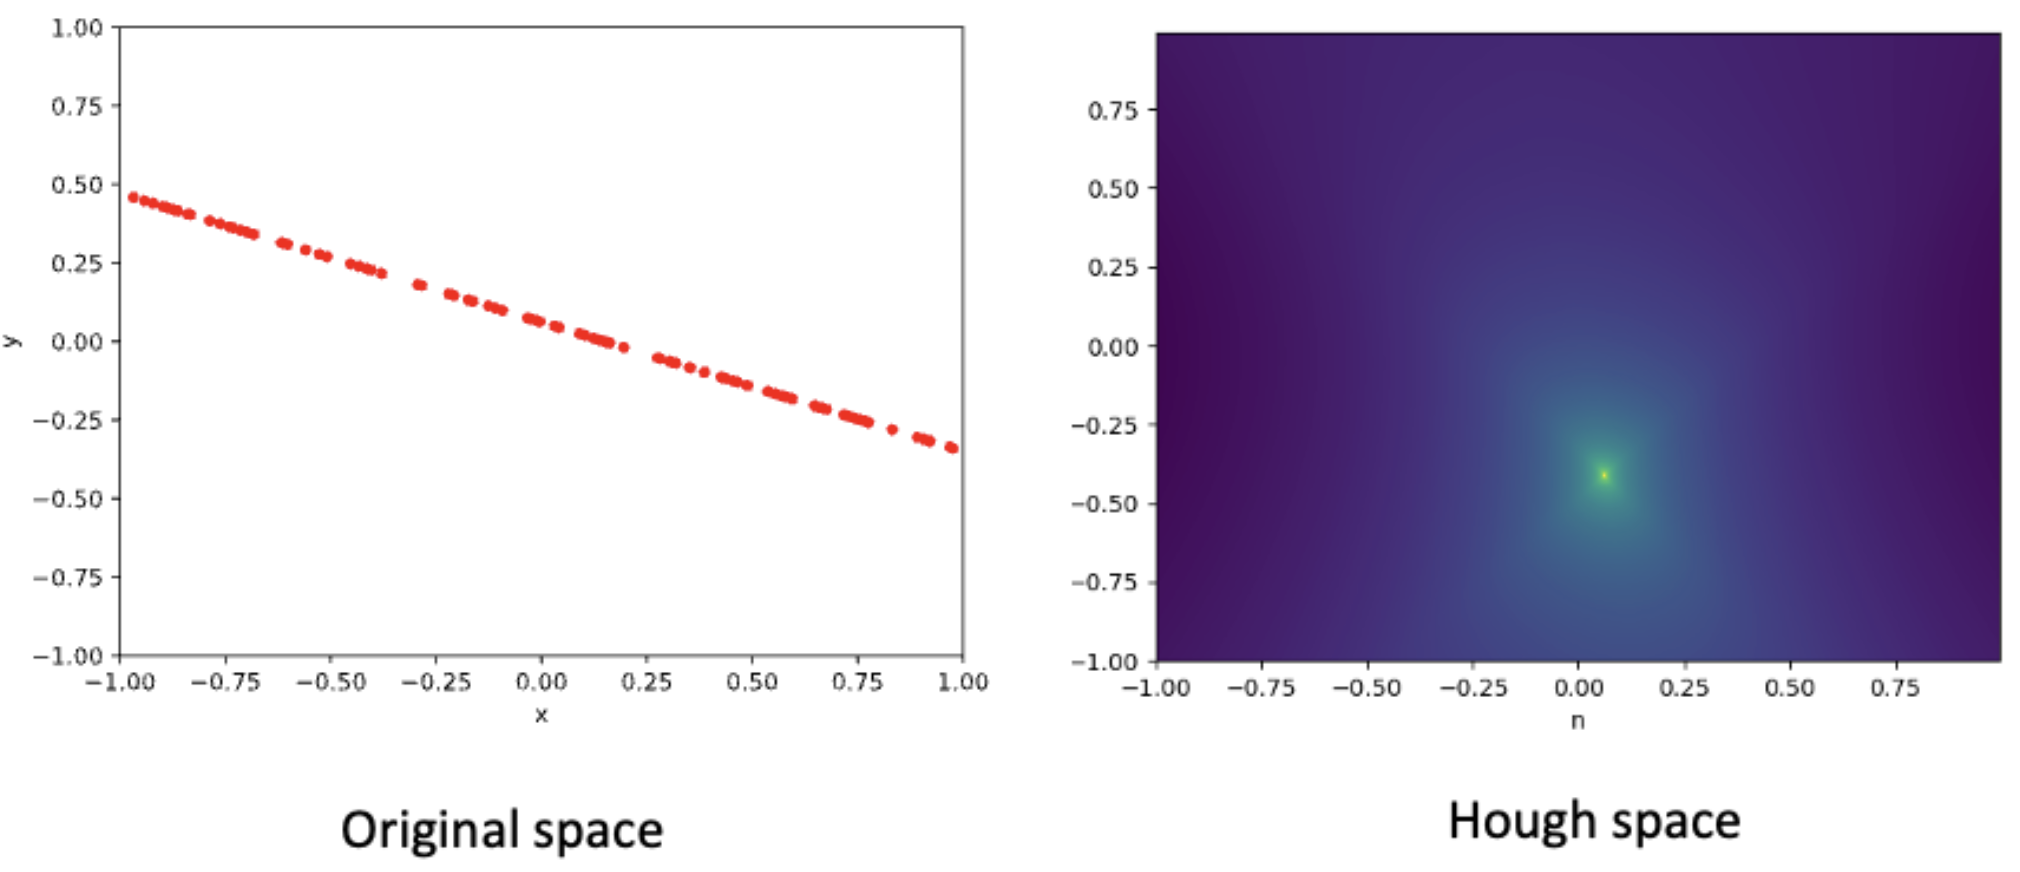
\includegraphics[width=0.8\textwidth]{figures/hough1.png}
    \caption{Hough Transform w/o Noise}
\end{figure}

\begin{figure}[htbp]
    \centering
    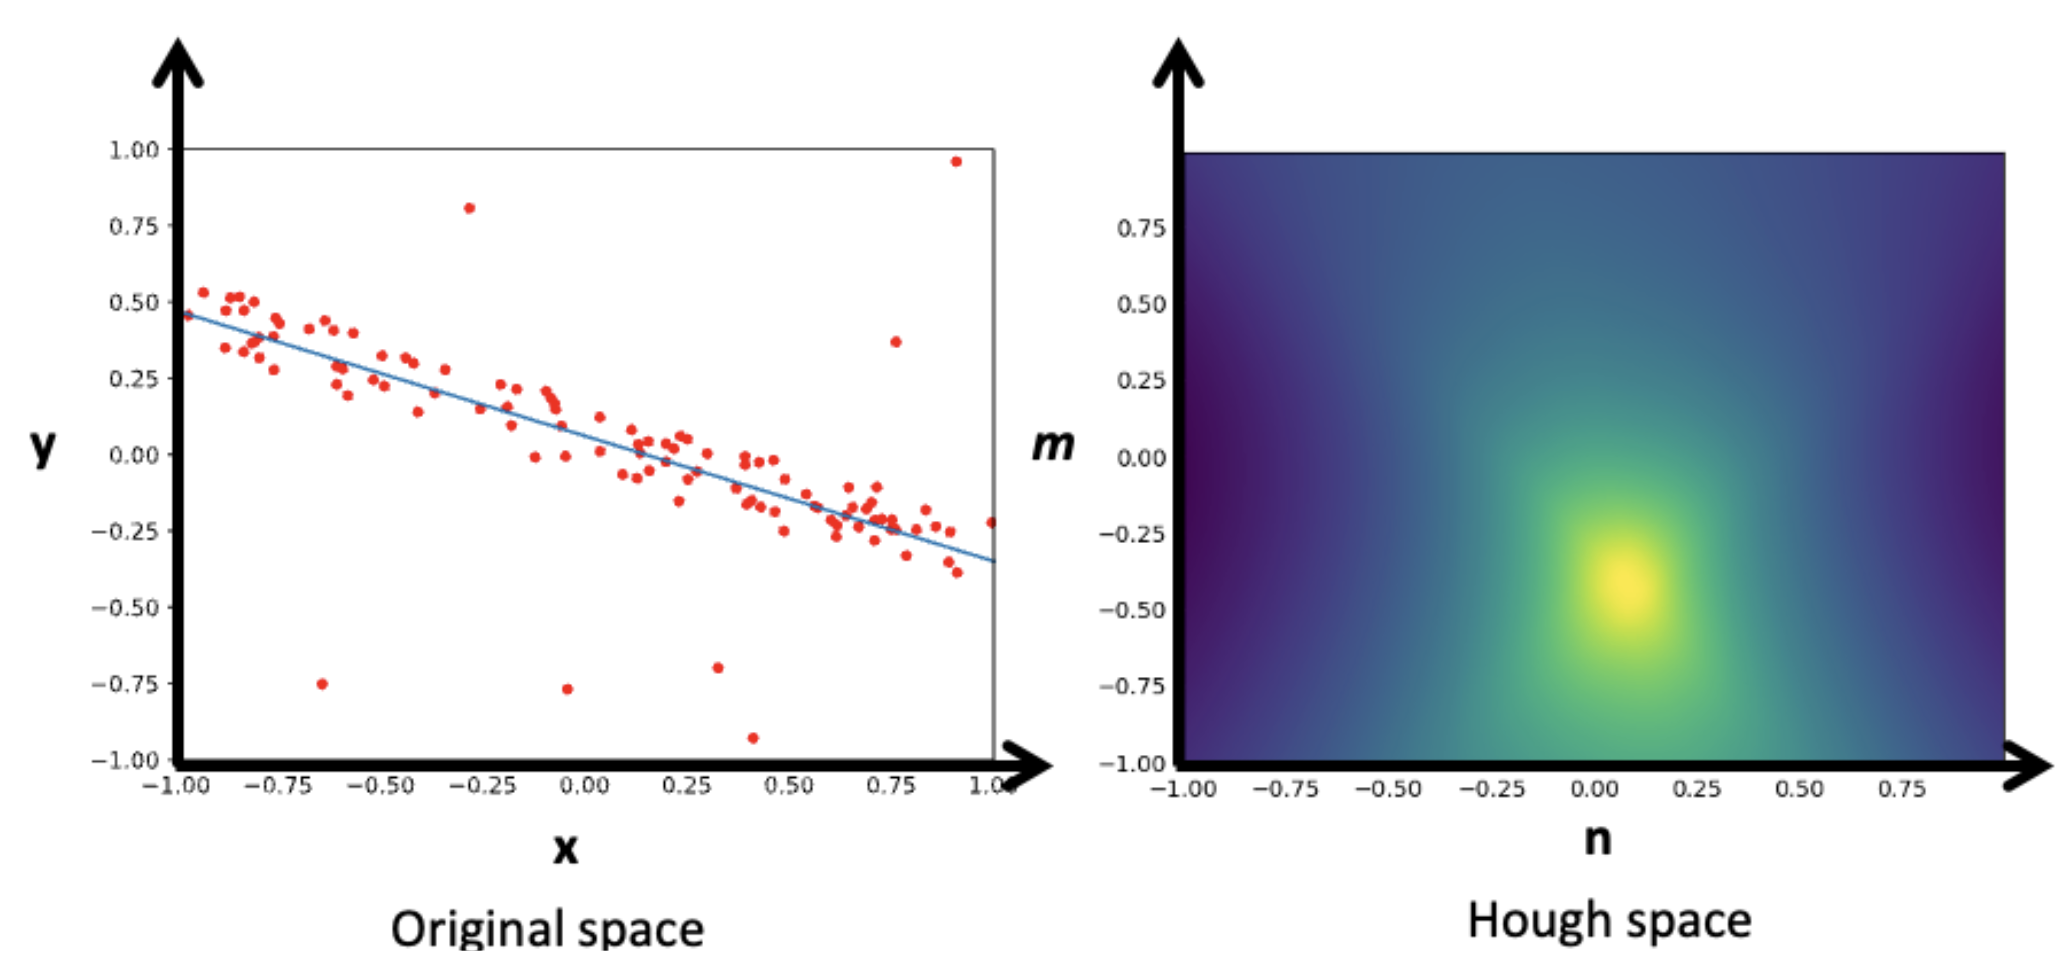
\includegraphics[width=0.8\textwidth]{figures/hough2.png}
    \caption{Hough Transform w/ Noise and Outliers}
\end{figure}




\chapter{Keypoint Detection}
(Corner Detection)

\begin{introduction}[Keywords]
    \item 角点检测 Corner Detection
    \item 结构张量 Structure Tensor
    \item 特征值分解 Eigenvalue Decomposition
    \item 等变性 Equivariance
    \item 尺度不变性 Scale Invariance
    \item Harris-Laplacian 检测器
    \item 高斯差分 Difference-of-Gaussians (DoG)
\end{introduction}

\begin{problem}
    What Points are Keypoints?
\end{problem}

\begin{enumerate}
    \item Repeatability: 可以在不同的图像中找到相同的点
    \item Saliency: 有趣的点
    \item Quantity: 量大管饱
    \item Accurate localization: 精确定位
\end{enumerate}
Corners 就是这样的 keypoints.




\section{The Basic Idea of Harris Corner}

\begin{figure}[htbp]
    \centering
    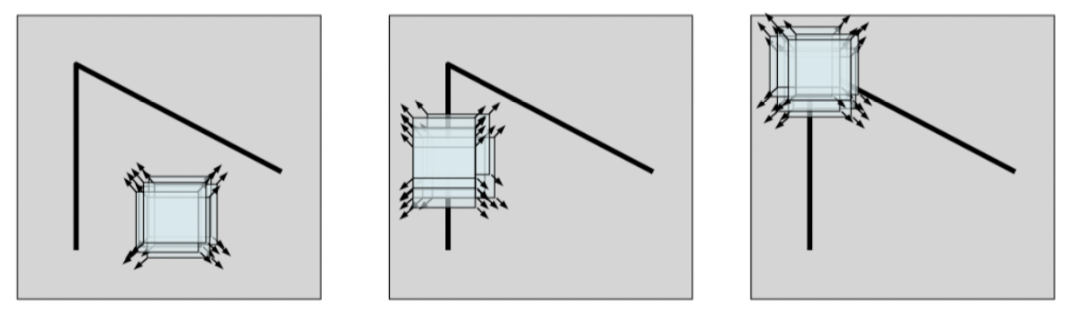
\includegraphics[width=0.8\textwidth]{figures/window_moving.png}
    \caption{移动窗口}    
\end{figure}

Move a window and explore intensity changes within the window.

Corner : significant change in all directions.

\section{Harris Corner}

一个 window,给定它的移动方向 $(u,v)$:

\begin{equation}
    \begin{aligned}
    E(u,v) &= \sum_{x,y} w(x,y) [I(x+u,y+v) - I(x,y)]^2\\
    &\approx \sum_{x,y} w(x,y) [I(x,y) + uI_x + vI_y - I(x,y)]^2\\
    &= \sum_{x,y} w(x,y) [uI_x + vI_y]^2\\
    &= w \ast \begin{bmatrix} u & v \end{bmatrix} \begin{bmatrix} I_x^2 & I_xI_y \\ I_xI_y & I_y^2 \end{bmatrix} \begin{bmatrix} u \\ v \end{bmatrix}\\
    &= \begin{bmatrix} u & v \end{bmatrix} \begin{bmatrix} w \ast I_x^2 & w \ast I_xI_y \\ w \ast I_xI_y & w \ast I_y^2 \end{bmatrix} \begin{bmatrix} u \\ v \end{bmatrix}\\
    &= \begin{bmatrix} u & v \end{bmatrix} R^{-1} \begin{bmatrix} \lambda_1 & 0\\ 0 & \lambda_2 \end{bmatrix} R \begin{bmatrix} u \\ v \end{bmatrix}\\
    &= \lambda_1 u_R^2 + \lambda_2 v_R^2
    \end{aligned}
\end{equation}

根据这两个特征值的大小可以判断这个点是不是角点.

\begin{figure}[htbp]
    \centering
    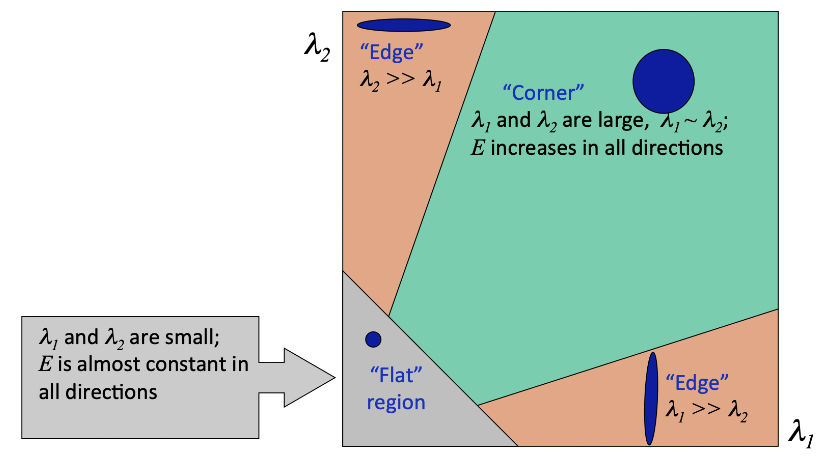
\includegraphics[width=0.6\textwidth]{figures/corner_map.png}
    \caption{特征值大小和这个点的是什么种类的点的关系}
\end{figure}
\begin{proposition}
    

这个点是角点一般需要满足:

\begin{itemize}
    \item $\lambda_1, \lambda_2>b$
    \item $\frac{1}{k}<\frac{\lambda_1}{\lambda_2}<k$
\end{itemize}

一个快速的判断公式:

\begin{equation}
\begin{aligned}
\theta&=\frac 12(\lambda_1\lambda_2-\alpha(\lambda_1+\lambda_2)^2)+\frac12(\lambda_1\lambda_2-2t)\\
&=\lambda_1\lambda_2-\alpha(\lambda_1+\lambda_2)^2-t\\
&=\det(R)-\alpha\text{Trace}(R)^2-t
\end{aligned}
\end{equation}

其中 $\alpha\in[0.04,0.06], t\in[0.01,0.03]$.

如果 $\theta$ 大于阈值, 则认为这个点是角点.
\end{proposition}
\begin{note}
Harris Corner 对平移和图像旋转是 equivariant的,对规模不是 equivariant 的.

为实现 rotation invariance, 可以用 Gaussian filter 来平滑图像, 使得角点不会因为旋转而改变.
\end{note}
\section{equivariant V.S. invariant}
\begin{definition}
    

\textbf{等变 (equivariant)}: $F(TX)=T(F(x))$,对于translation和rotation是等变的.

\textbf{不变 (invariant)}: $F(T(X))=F(X)$,也就是对于不同位置导出的角点还是那样,所以其实我们想要的是等变,也就是对于不同位置导出的角点做了同样的变化.
\end{definition}

\begin{problem}
    How to prove Harris detector is equivariant?
\end{problem}


只要说明角点检测函数也是equivariant即可.

角点检测函数包括了求导和卷积两个操作,显然求导是equivariant的,因为导数会随着trans和rot做相同的变化.

很有趣的是卷积也是equivariant的:当你的filter function是各向同性的,那么这个卷积就是equivariant的;但是如果是一个椭圆形的window,那这个卷积就不是equivariant的了.

\begin{figure}[htbp]
    \centering
    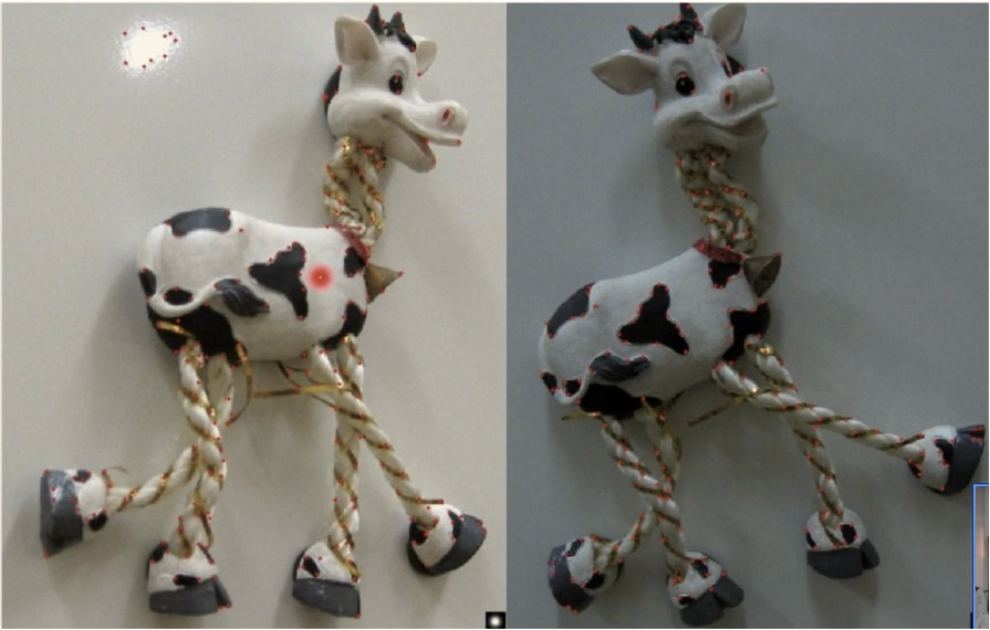
\includegraphics[width=0.6\textwidth]{figures/light_invariant.png}
    \caption{Illumination invariant}
\end{figure}
\begin{remark}
    这个高光说明不是环境 Illumination Invariant的
\end{remark}


\begin{problem}
    How to do NMS with corner-response-function?
\end{problem}


一个简单的想法:

先给出一个阈值,把所有response排序,成为一个list,从上到下按顺序把这个pixel周围的大于阈值的踢出list.
这个跟之前的NMS区别在于之前需要一条边,现在只需要一个点,那么现在比之前踢出的像素点更多.

\section{Scale Invariant Detectors}

这个不讲了?下次看看

Harris-Laplacian, SIFT (Lowe)

\printbibliography[heading=bibintoc, title=\ebibname]
\end{document}
